\documentclass{article}
\usepackage{graphicx}
\title{Historical perspective of programming languages}
\author{by Emokhor Daniel}
\begin{document}
	\pagenumbering{gobble}
	\maketitle
	\newpage
	In this presentation I will be looking at these 5 programming languages, namely:
	\begin{itemize}
		\item HTML (HYPER TEXT MARKUP LANGUAGE)
		\item JAVA
		\item C++
		\item C
		\item JAVASCRIPT
	\end{itemize}
    \newpage
    \maketitle \textbf{ HTML- THE HISTORY}
    \begin{itemize}
        \item Also known as “Hypertext markup language”, It was originally proposed as “html tags” by tim berners-lee in 1993.
        \item But it was in late 1994 that a html working group was formed which later created “html 2” the following year. 
        \item It is a markup language (markup languages are languages that explain documents in ways that they are easily understandable) that a web browser or developer uses to develop or interpret text into audio or video files in a web page.
   \end{itemize}
\newpage
\begin{figure}
	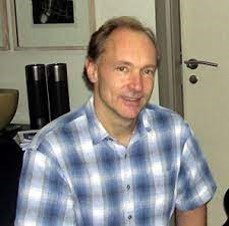
\includegraphics[width=\linewidth]{Picture1}
	\caption{Tim berners-lee, creator of HTML programming language}
\end{figure}


   \newpage
   \maketitle \textbf{What can be developed with html}
   \begin{itemize}
     	\item WEB PAGES
	    \item ONLINE-GAME DEVELOPMENT
   \end{itemize}
\newpage
\maketitle \textbf{Available Integrated development environment for html}
\begin{itemize}
	\item Visual stuio code
    \item Pycharm
	\item Komodo edit
	\item Netbeans
	\item Light table
	
\end{itemize}
\newpage
\maketitle \textbf{JAVA PROGRAMMING- THE HISTORY AND FOUNDER}
\begin{itemize} 
	\item Java was started by James Gosling in 1991, in fact he got the idea for the name from a green tea brand from thailand. it was originally known as oak, then later changed to green before it was finally named Java.
\item It was initially set up for interactive television but due to the low level of television technology at the time, it was not implemented in the industry.
\item The first release was in 1996 by Sun microsystems.
\end{itemize}


    
    

\end{document}	